\documentclass{standalone}
\usepackage{tikz}
\usetikzlibrary{calc}
\begin{document}
    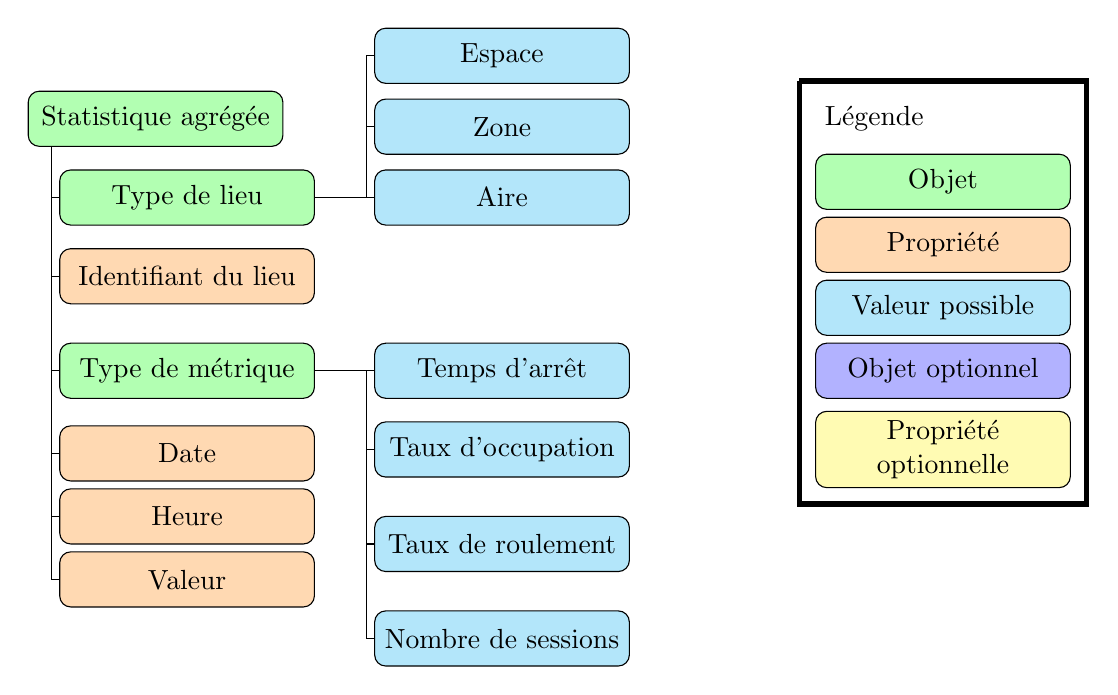
\begin{tikzpicture}
        \tikzstyle {objet} = [rectangle, rounded corners, text width=3cm, minimum height=0.7cm,text centered,  draw=black, fill=green!30]
        \tikzstyle {objet_opt} = [rectangle, rounded corners, text width=3cm, minimum height=0.7cm,text centered,  draw=black, fill=blue!30]
        \tikzstyle {propriete} = [rectangle, rounded corners, text width=3cm, minimum height=0.7cm,text centered,  draw=black, fill=orange!30]
        \tikzstyle{propriete_opt} =[rectangle, rounded corners, text width=3cm, minimum height=0.7cm,text centered,  draw=black, fill=yellow!30]
        \tikzstyle{enumeration} = [rectangle, rounded corners, text width=3cm, minimum height=0.7cm,text centered,  draw=black, fill=cyan!30]
        \node (statistique) [objet]{Statistique agrégée};
        \node (curb_place_type) [objet,below of=statistique,xshift=0.4cm]{Type de lieu};
        \node (aire) [enumeration, right of=curb_place_type,xshift=3cm]{Aire};
        \node (zone) [enumeration, above of=aire,yshift=-0.1cm]{Zone};
        \node (place) [enumeration, above of=zone,yshift=-0.1cm]{Espace};
        \node (curb_place_id) [propriete, below of=curb_place_type]{Identifiant du lieu};
        \node (type_metrique) [objet, below of=curb_place_id,yshift=-0.2cm]{Type de métrique};
        \node (temps_arret) [enumeration,right of=type_metrique,xshift=3cm]{Temps d'arrêt};
        \node (taux_occupation) [enumeration,below of=temps_arret]{Taux d'occupation};
        \node (taux_roulement) [enumeration, below of=taux_occupation,yshift=-0.2cm]{Taux de roulement};
        \node (nombre_sessions) [enumeration, below of=taux_roulement,yshift=-0.2cm]{Nombre de sessions};
        \node (date) [propriete,below of=type_metrique,yshift=-0.05cm]{Date};
        \node (heure) [propriete, below of=date,yshift=0.2cm]{Heure};
        \node (valeur) [propriete,below of=heure,yshift=0.2cm]{Valeur};
        \draw (curb_place_type.west) -| ($(statistique.south -| curb_place_type.west) + (-0.1,0)$);
        \draw (curb_place_type.west) -| ++(-0.1,-0.1) |- (curb_place_id.west);
        \draw (curb_place_id.west) -|++(-0.1,-0.1) |- (type_metrique.west);
        \draw (type_metrique.west) -|++(-0.1,-0.1) |- (date.west);
        \draw (date.west)  -|++(-0.1,-0.1) |- (heure.west);
        \draw (heure.west) -|++(-0.1,-0.1) |- (valeur.west);
        \draw (curb_place_type.east) -- (aire.west);
        \draw (aire.west) -| ++(-0.1,0.1) |- (zone.west);
        \draw (zone.west) -| ++(-0.1,0.1) |- (place.west);
        \draw (type_metrique.east) -- (temps_arret.west);
        \draw (temps_arret.west) -| ++(-0.1,-0.1) |- (taux_occupation.west);
        \draw (taux_occupation.west) -| ++(-0.1,-0.1) |- (taux_roulement.west);
        \draw (taux_roulement.west) -| ++(-0.1,-0.1) |- (nombre_sessions.west);
        \node (legend) [text width =3cm,right of=statistique, xshift=9cm]{Légende};
        \node (obj_leg) [objet, below of=legend,yshift=0.2cm]{Objet};
        \node (prop_leg) [propriete, below of=obj_leg,yshift=0.2cm]{Propriété};
        \node (enum_leg) [enumeration , below of=prop_leg,yshift=0.2cm]{Valeur possible};
        \node (obj_opt_leg) [objet_opt, below of=enum_leg,yshift=0.2cm]{Objet optionnel};
        \node (propriete_opt_leg) [propriete_opt, below of=obj_opt_leg]{Propriété optionnelle};
        \coordinate (legend_box_top_left) at ($(legend.north west) + (-0.2,0.2)$);
        \coordinate (legend_box_bottom_right) at ($(propriete_opt_leg.south east) + (0.2,-0.2)$);
        \draw[line width=2pt] (legend_box_top_left) -| (legend_box_bottom_right) -| (legend_box_top_left);
    \end{tikzpicture}
\end{document}